\chapter{生殖发育与开花调控}\label{ch:b2:plant-flowering}

一位菊花种植者可以通过调节灯光，让温室里的菊花赶在圣诞节
或复活节开花；春季播种的冬小麦则从不开花，
因为它没有经历过低温；一株苍耳只要经历过
一个比临界长度更长的夜晚，
此后无论发生什么，它都注定要开花。
植物没有日历，却有生物钟、温度计和光照计，
每年它都会依据这些证据，
把一直在长叶的\omterm{def:b2:plant-meristems:meristem}{分生组织}转变为会形成花的\omterm{def:b2:plant-meristems:meristem}{分生组织}。
本章沿着这一决定展开：从测量夜长的叶片，
到改变发育程序的\omterm{def:b2:plant-meristems:meristem}{分生组织}，
再到由基因编码所构建的花，
以及生命周期另一端的逆向转变——\omterm{def:b2:angiosperm-reproduction:seed}{种子}在得知季节合适之前，
不会萌发。

\section{向开花的转变}

\begin{definition}[成花转变与成花诱导]\label{def:b2:plant-flowering:transition}
\index{成花转变}\index{成花诱导}\index{花序分生组织}
营养\omterm{def:b2:plant-meristems:meristem}{茎尖分生组织}在每个叶腋中产生一个芽，
无限地制造叶片。在\emph{成花转变}时，它变成
\emph{花序\omterm{def:b2:plant-meristems:meristem}{分生组织}}，产生苞片，并在苞片的腋内形成
\emph{花\omterm{def:b2:plant-meristems:meristem}{分生组织}}；每个花\omterm{def:b2:plant-meristems:meristem}{分生组织}都是有限生长的：
它依次形成萼片、花瓣、\omterm{def:b2:angiosperm-reproduction:flower}{雄蕊}和\omterm{def:b2:angiosperm-reproduction:flower}{心皮}，然后停止生长。
这一变化由\emph{成花诱导}触发——诱导信号或来自叶片，
或产生于植物自身的生理过程，它开启\omterm{def:b2:plant-meristems:meristem}{分生组织}的身份基因。
一年生植物开花一次便死亡；
多年生植物每年从部分\omterm{def:b2:plant-meristems:meristem}{分生组织}开花，其余\omterm{def:b2:plant-meristems:meristem}{分生组织}则保持营养生长。
开花时间决定\omterm{def:b2:plant-life-cycles:heterospory}{花粉}能否遇到\omterm{def:b2:plant-life-cycles:heterospory}{花粉}、\omterm{def:b2:angiosperm-reproduction:seed}{种子}能否在霜冻来临前成熟，
以及花朵是否在\omterm{def:b2:angiosperm-reproduction:pollination}{传粉}者飞来时绽放：
这一性状受到强烈的选择，
植物已演化出多种读取季节信号的方式。
\end{definition}

\begin{proposition}[光周期现象：植物测量夜长]\label{prop:b2:plant-flowering:photoperiod}
\index{光周期现象}\index{短日植物}\index{长日植物}\index{光敏色素}
许多植物对日长作出反应而开花。\emph{\omterm{prop:b2:plant-flowering:photoperiod}{短日植物}}（
菊花、大豆、水稻、苍耳）在日长短于临界长度时开花，即在秋季或春季；
\emph{\omterm{prop:b2:plant-flowering:photoperiod}{长日植物}}（菠菜、小麦、三叶草、
\emph{Arabidopsis}）在日长长于临界长度时开花，即在初夏；
\emph{日中性植物}（番茄、玉米）则在长到足够大时开花。
实际上，植物所测量的是连续不间断的\emph{夜长}：
\omterm{prop:b2:plant-flowering:photoperiod}{短日植物}也就是长夜植物，
在长夜中间照一次光就会抵消其效应，
而在长日中间的一段黑暗则没有这种作用。
测量在\emph{叶片}中进行，依靠色素\emph{\omterm{prop:b2:plant-flowering:photoperiod}{光敏色素}}——
一种蛋白质，每捕获一个光子，
它就在吸收红光的形式与吸收远红光的形式之间转换，
因此其状态记录了光照，
测量参照一个内部的\emph{生物钟}，
周期约为二十四小时：只有当光照恰好与生物钟的某一特定时相重合时，
开花才会被触发，
而这只在合适的日长下才会发生。
\end{proposition}
\begin{proof}[证据]
Garner 和 Allard（1920）发现，一个\omterm{def:b2:genome-diversification:mutation}{突变}烟草
只在冬季温室的短日照下开花；夏季间隔播种的大豆
则全部在九月一同开花：决定开花时间的是日长，
而不是植株的年龄或温度。Hamner 和 Bonner（1938）
以苍耳证明，一个长夜便已足够；
夜间中途的一分钟光照即可消除效应，
而缩短白昼、夜长不变，则不能诱导开花。
Borthwick 和 Hendricks（1952）发现，最有效的光是红光，
紧随红光之后照射远红光则会将其抵消——
这正是\omterm{prop:b2:plant-flowering:photoperiod}{光敏色素}的特征，该色素于 1959 年被分离出来。
将一片已被诱导的叶片嫁接到未被诱导的植株上，
能使整株植物开花：叶片输出了某种信号。
\end{proof}

\begin{omfigure}
\begin{tikzpicture}[every node/.style={font=\scriptsize}]
  \foreach \y/\lab/\res in {3.6/{长日照，短夜}/{不开花}, 2.7/{短日照，长夜}/{开花}, 1.8/{长夜被一次闪光打断}/{不开花}, 0.9/{长日照被黑暗打断}/{不开花}} {
    \node[anchor=east, align=right] at (-0.2,\y) {\lab};
    \node[anchor=west, omThm] at (8.6,\y) {\res};
  }
  % bars: 24 h = 8 cm; light yellow, dark grey
  \fill[omExo!30] (0,3.4) rectangle (8,3.8); \fill[yellow!50!orange!40] (0,3.4) rectangle (5.4,3.8);
  \fill[omExo!30] (0,2.5) rectangle (8,2.9); \fill[yellow!50!orange!40] (0,2.5) rectangle (3.0,2.9);
  \fill[omExo!30] (0,1.6) rectangle (8,2.0); \fill[yellow!50!orange!40] (0,1.6) rectangle (3.0,2.0); \fill[yellow!50!orange!40] (5.4,1.6) rectangle (5.55,2.0);
  \fill[omExo!30] (0,0.7) rectangle (8,1.1); \fill[yellow!50!orange!40] (0,0.7) rectangle (5.4,1.1); \fill[omExo!30] (2.6,0.7) rectangle (2.9,1.1);
  \draw[thick, ->] (0,0.3) -- (8.2,0.3); \foreach \x/\l in {0/0,2/6,4/12,6/18,8/24} \draw (\x,0.35) -- (\x,0.25) node[below] {\l};
  \node[below] at (4,-0.05) {小时};
  \draw[dashed, omDef] (5.4,0.3) -- (5.4,4.0); \node[omDef, above] at (5.4,4.0) {临界夜长};
\end{tikzpicture}

{\small Hamner 和 Bonner 的苍耳，一种\omterm{prop:b2:plant-flowering:photoperiod}{短日植物}。它
在夜长超过临界长度后开花；夜间中途一分钟的光照
会抵消诱导，而白昼中的一段黑暗则不会。
植物测量的是夜长。}
\end{omfigure}

\begin{definition}[成花素]\label{def:b2:plant-flowering:florigen}
\index{成花素}\index{FLOWERING LOCUS T}
叶片输出的这一信号于 1937 年被命名为\emph{成花素}，
七十年后被鉴定为一种小蛋白质，即基因
\emph{FLOWERING LOCUS T}（FT）的产物。在叶片中，
生物钟与\omterm{prop:b2:plant-flowering:photoperiod}{光敏色素}共同作用，只有在日长合适时才开启 FT
（在\omterm{prop:b2:plant-flowering:photoperiod}{长日植物}\emph{Arabidopsis}中，当光照与生物钟控制的激活因子 CONSTANS 的午后峰值重合时）；
FT 蛋白进入韧皮部，随糖流输送至茎尖，
并在那里与一种伙伴蛋白一起，
开启使\omterm{def:b2:plant-meristems:meristem}{分生组织}发生转变的基因。
同一种蛋白也是\omterm{prop:b2:plant-flowering:photoperiod}{短日植物}水稻的成花素，
只是其中的生物钟以相反的方式连接它。
嫁接实验、蛋白质在韧皮部中的运输，
以及在叶片特异性启动子驱动下表达 FT 的植株能够开花，
三者结论一致：开花在叶片中决定，
在芽中执行。
\end{definition}

\begin{omfigure}
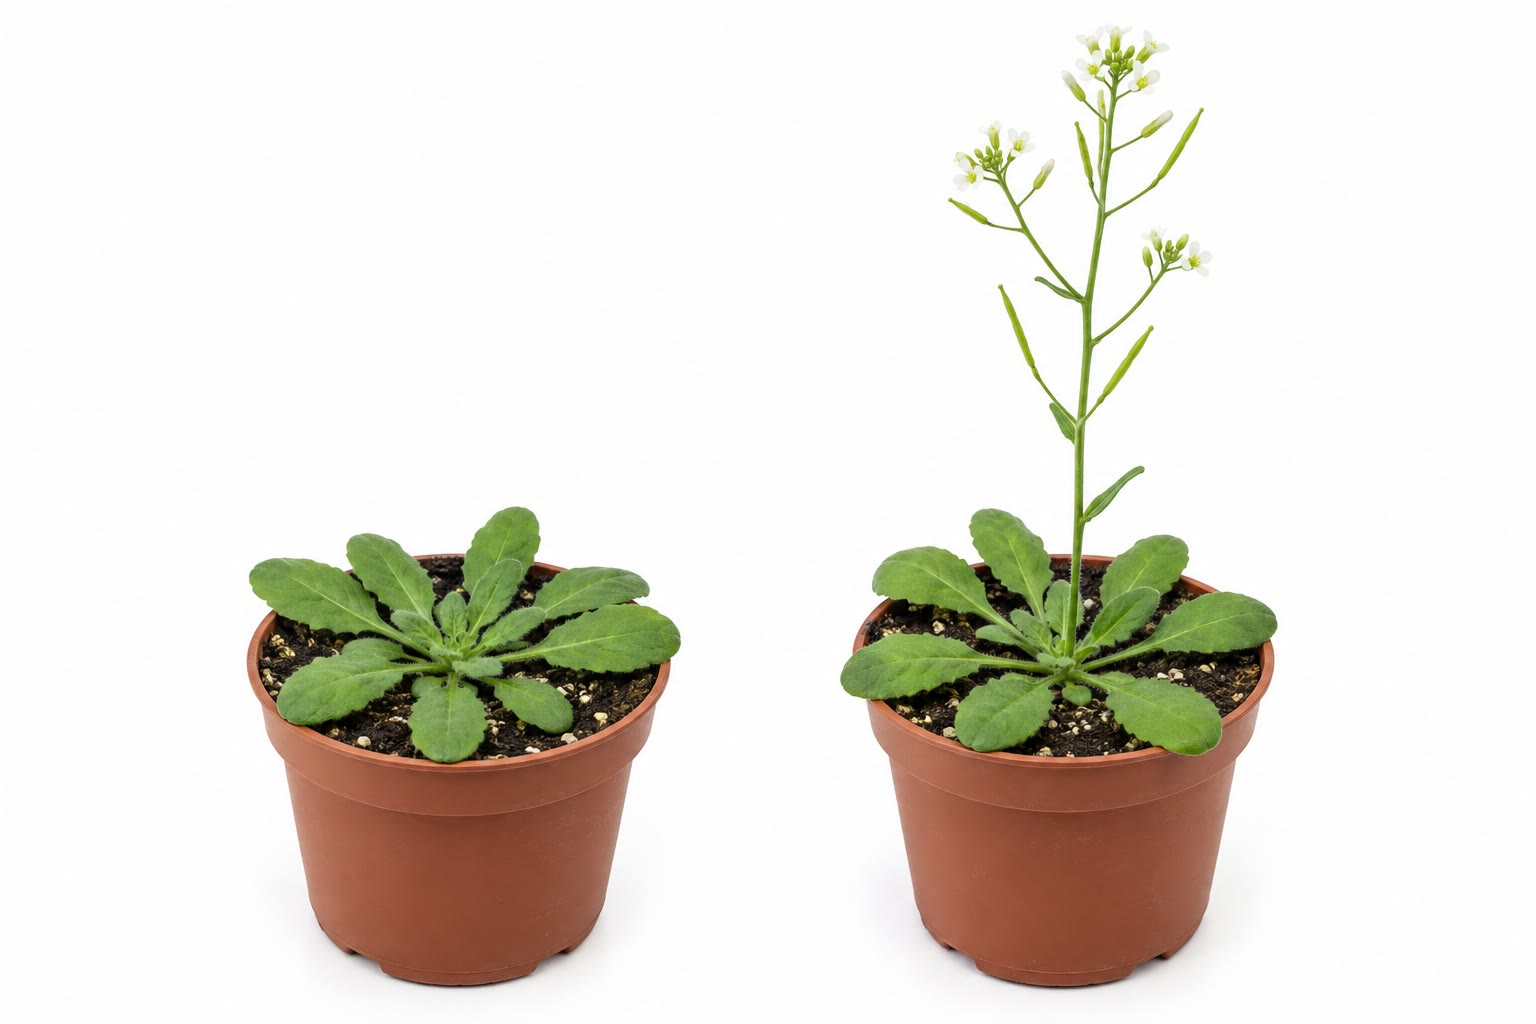
\includegraphics[width=0.58\linewidth]{images/book4/ai/b4-14-arabidopsis-daylength.jpg}

{\small \emph{Arabidopsis}，\omterm{prop:b2:plant-flowering:photoperiod}{长日植物}：短日照下
为一丛莲座叶；移至长日照后，
数周内抽薹开花。}
\end{omfigure}

\begin{proposition}[春化作用：植物计算寒冷]\label{prop:b2:plant-flowering:vernalisation}
\index{春化作用}\index{FLOWERING LOCUS C}
冬性谷物、二年生植物（胡萝卜、卷心菜、毛地黄）以及许多
寒冷气候下的多年生植物须先经历数周低温才会开花
——\emph{\omterm{prop:b2:plant-flowering:vernalisation}{春化作用}}——
这保证了秋季萌发的植物等到春天，
而不是在霜冻中开花。低温由\omterm{def:b2:plant-meristems:meristem}{分生组织}本身感知，
而非由叶片感知；它不能被任何其他处理替代；
其效应会记忆在植物此后的生长中，
经数百次细胞分裂保持，但不会通过
\omterm{def:b2:meiosis-heredity:meiosis}{减数分裂}传递——每粒\omterm{def:b2:angiosperm-reproduction:seed}{种子}都从未春化开始。在\emph{Arabidopsis}中
这一记忆由一个基因承载，即\emph{FLOWERING LOCUS C}（FLC），其产物
抑制开花：数周低温通过在染色质上
覆盖抑制性标记而使其逐步沉默，此沉默
在每次分裂时被复制，并在胚胎中被清除。植物
因此随时间\emph{整合}低温的累积——几天的低温不算数——
而缺少 FLC 的\omterm{def:b2:genome-diversification:mutation}{突变}体无需冬季。
\end{proposition}

\begin{theorem}[为什么整合能防止假春天]\label{thm:b2:plant-flowering:integration}
设抑制因子每个低温日以恒定速率 $\alpha$ 被沉默，
于是经过 $n$ 个低温日后仍保持活性的比例为
$f_n = e^{-\alpha n}$，且当 $f < f_c$ 时允许开花。
所需低温日数为 $n_c = \ln(1/f_c)/\alpha$，
由于沉默是稳定的，低温日无需连续——
起作用的是它们的总数。若植物的 $n_c = 40$
则不会被一月中两周的解冻或
十月的寒潮欺骗；若植物只感知当前温度，
它将在第一个温暖的星期开花。同样的整合配合一个
阈值，便是植物在作出决定前读取累积日长的方式，
两者都是系统对信号的
\emph{积分}而非瞬时值作出响应的例子。
\end{theorem}
\begin{proof}
若每个低温日沉默剩余活性拷贝（或尚未标记的染色质）的
比例 $\alpha$，则活性比例
满足 $f_{n+1} = (1 - \alpha)f_n \approx e^{-\alpha}f_n$，
从而 $f_n = e^{-\alpha n}$，其中 $n$ 为低温日的计数；
不等式 $e^{-\alpha n} < f_c$ 给出 $n > \ln(1/f_c)/\alpha$。
非低温日既不增加也不减少，
因为标记是稳定的，故只有总数有意义。
\end{proof}

\section{构建花：ABC 模型}

\begin{proposition}[ABC 模型]\label{prop:b2:plant-flowering:abc}
\index{ABC 模型}\index{同源异型基因!花}
花\omterm{def:b2:plant-meristems:meristem}{分生组织}形成四轮同心的花轮：萼片、花瓣、
\omterm{def:b2:angiosperm-reproduction:flower}{雄蕊}、\omterm{def:b2:angiosperm-reproduction:flower}{心皮}。它们的身份由三类
\emph{同源异型基因}决定，它们在部分重叠的环带中起作用：第 1 轮中单独的 A 类
基因产生萼片；第 2 轮中 A 类与 B 类共同作用产生花瓣；
第 3 轮中 B 类与 C 类共同作用产生\omterm{def:b2:angiosperm-reproduction:flower}{雄蕊}；第 4 轮中单独的 C 类产生
\omterm{def:b2:angiosperm-reproduction:flower}{心皮}。A 类与 C 类相互抑制，因此一方缺失时，
另一方会扩展至整朵花。这些规则可预测每一种单\omterm{def:b2:genome-diversification:mutation}{突变}体：
缺失 B 类，花为萼片—萼片—\omterm{def:b2:angiosperm-reproduction:flower}{心皮}—\omterm{def:b2:angiosperm-reproduction:flower}{心皮}；
缺失 C 类，花为萼片—花瓣—花瓣—萼片，花内还会再套一朵花
，因为 C 类同时终止\omterm{def:b2:plant-meristems:meristem}{分生组织}；缺失 A 类，花为
\omterm{def:b2:angiosperm-reproduction:flower}{心皮}—\omterm{def:b2:angiosperm-reproduction:flower}{雄蕊}—\omterm{def:b2:angiosperm-reproduction:flower}{雄蕊}—\omterm{def:b2:angiosperm-reproduction:flower}{心皮}。这些基因大多编码
同一家族（MADS-box）的\omterm{prop:b2:cell-differentiation:transcriptional}{转录因子}，另有第四类 E 类基因，
三种功能均需要它；若在叶片中同时表达 B 类与 C 类基因，
叶片便转变为类似\omterm{def:b2:angiosperm-reproduction:flower}{雄蕊}的器官。园林中的
重瓣花——玫瑰、牡丹、山茶——都是 C 类\omterm{def:b2:genome-diversification:mutation}{突变}体，
其\omterm{def:b2:angiosperm-reproduction:flower}{雄蕊}变成了额外的花瓣。
\end{proposition}
\begin{proof}[证据]
Coen 和 Meyerowitz（1991）比较了
\emph{Arabidopsis}与金鱼草的同源异型\omterm{def:b2:genome-diversification:mutation}{突变}体：两者中，三类\omterm{def:b2:genome-diversification:mutation}{突变}
各自都使相邻两轮发生转变，且转变的配对相同，
\omterm{def:b2:genome-diversification:mutation}{突变}体组合的表现与模型预测一致（三重\omterm{def:b2:genome-diversification:mutation}{突变}体只产生叶片）。
\omterm{def:b2:asexual-reproduction:clone}{克隆}结果表明，这些基因是\omterm{prop:b2:cell-differentiation:transcriptional}{转录因子}，
并在预测的环带中表达；将 B 类基因置于在四轮中均活跃的启动子之下，
所得花为
花瓣—花瓣—\omterm{def:b2:angiosperm-reproduction:flower}{雄蕊}—\omterm{def:b2:angiosperm-reproduction:flower}{雄蕊}。
\end{proof}

\begin{omfigure}
\begin{tikzpicture}[every node/.style={font=\scriptsize}]
  % four whorls as columns
  \foreach \x/\w in {0/{第 1 轮}, 2.2/{第 2 轮}, 4.4/{第 3 轮}, 6.6/{第 4 轮}} \node[above] at (\x+0.9,3.3) {\w};
  \fill[omDef!35] (0,2.4) rectangle (4.2,3.1); \node at (2.1,2.75) {A};
  \fill[omProp!40] (2.2,1.6) rectangle (6.4,2.3); \node at (4.3,1.95) {B};
  \fill[omThm!30] (4.4,0.8) rectangle (8.6,1.5); \node at (6.5,1.15) {C};
  \foreach \x/\o in {0/萼片, 2.2/花瓣, 4.4/雄蕊, 6.6/心皮} \node[below, align=center] at (\x+0.9,0.6) {\o};
  \node[anchor=west, align=left] at (9.2,3.0) {野生型：A、AB、BC、C};
  \node[anchor=west, align=left] at (9.2,2.3) {无 B：萼片、萼片、心皮、心皮};
  \node[anchor=west, align=left] at (9.2,1.6) {无 C：萼片、花瓣、花瓣、萼片……};
  \node[anchor=west, align=left] at (9.2,0.9) {无 A：心皮、雄蕊、雄蕊、心皮};
\end{tikzpicture}

{\small ABC 模型。三类基因以部分重叠的环带设定四种器官身份；
失去其中一类会使两个花轮发生转变，
所得\omterm{def:b2:genome-diversification:mutation}{突变}花与预测完全一致。}
\end{omfigure}

\begin{omfigure}
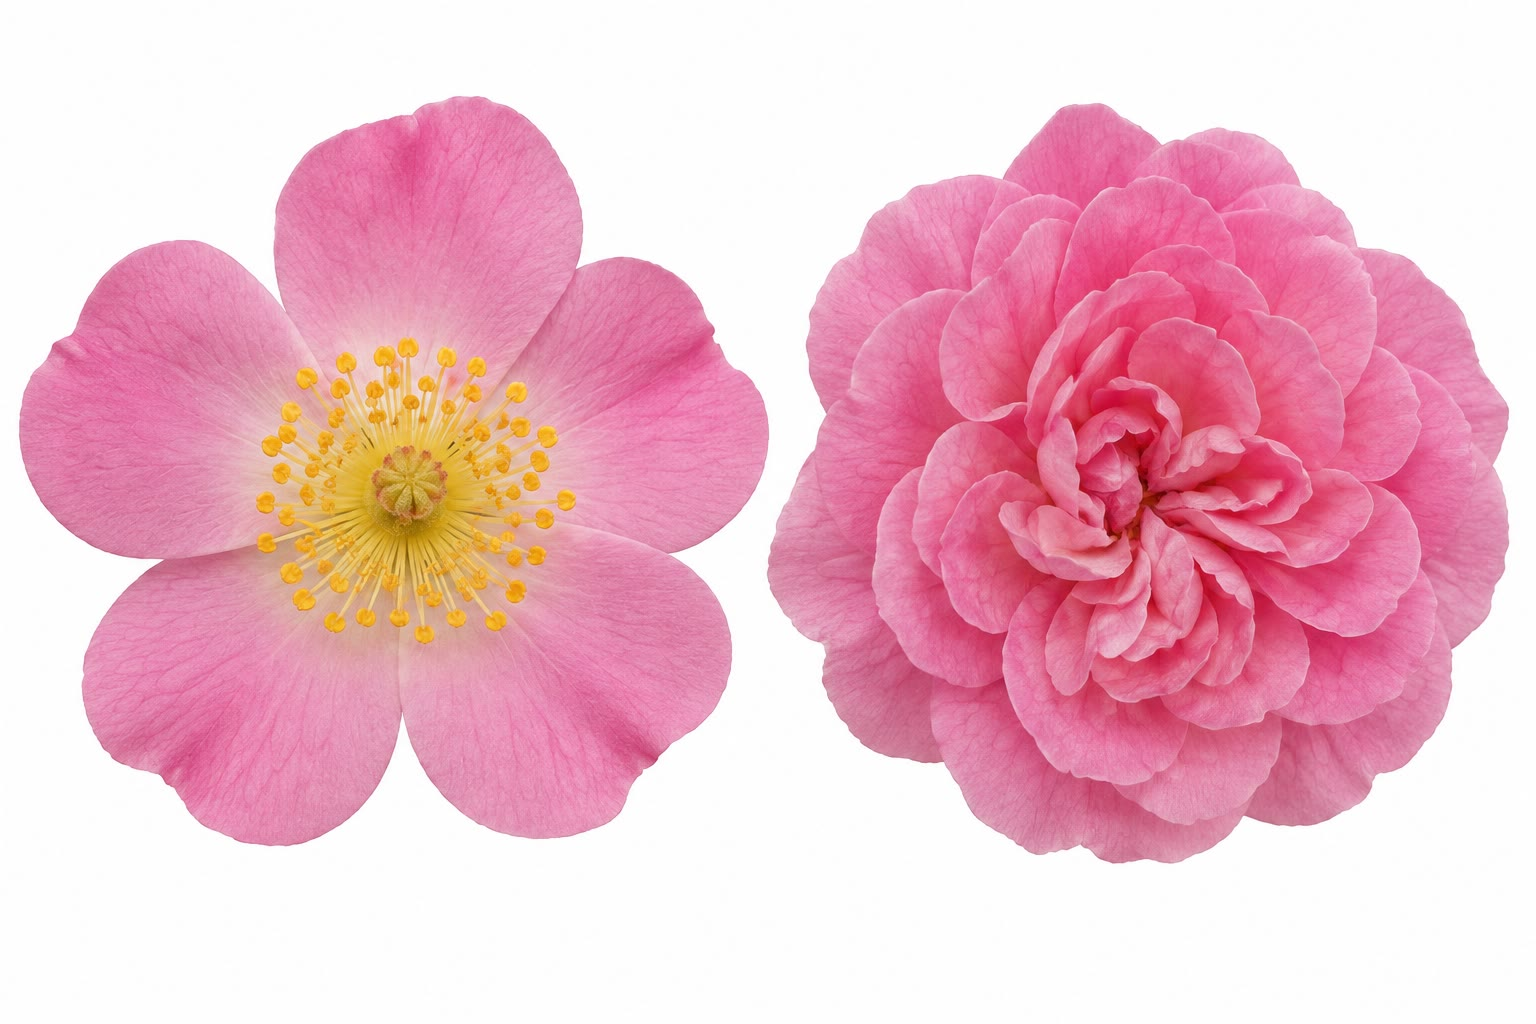
\includegraphics[width=0.58\linewidth]{images/book4/ai/b4-14-double-flower.jpg}

{\small 野生型花与重瓣型花并列：\omterm{def:b2:angiosperm-reproduction:flower}{雄蕊}已变成花瓣——
一个 C 类\omterm{def:b2:genome-diversification:mutation}{突变}体，园艺工人数百年来对其加以选育，
而人们直到后来才知道它为何是重瓣。}
\end{omfigure}

\section{休眠与萌发}

\begin{definition}[种子休眠]\label{def:b2:plant-flowering:dormancy}
\index{休眠!种子}\index{脱落酸}\index{赤霉素}\index{层积处理}
活\omterm{def:b2:angiosperm-reproduction:seed}{种子}若在本可支持生长的条件下仍不萌发，
则称为\emph{\omterm{def:b2:angiosperm-reproduction:seed}{休眠}的}。\omterm{def:b2:angiosperm-reproduction:seed}{休眠}在\omterm{def:b2:angiosperm-reproduction:seed}{种子}成熟期间施加，
由\emph{脱落酸}（ABA）引起，它同时促使贮藏物质积累，
并使胚干燥。\omterm{def:b2:angiosperm-reproduction:seed}{休眠}由\omterm{def:b2:angiosperm-reproduction:seed}{种皮}维持（不透水、不透氧，
机械地约束胚），或由胚自身的状态维持。
\omterm{def:b2:angiosperm-reproduction:seed}{休眠}的打破依靠标志不利季节结束的信号：
数周的低温与潮湿（\emph{层积处理}，即\omterm{def:b2:angiosperm-reproduction:seed}{种子}的
\omterm{prop:b2:plant-flowering:vernalisation}{春化作用}），光照（对必须靠近地表的小\omterm{def:b2:angiosperm-reproduction:seed}{种子}，
由\omterm{prop:b2:plant-flowering:photoperiod}{光敏色素}感知），或黑暗、交变温度，
雨水浸出抑制剂、土壤或消化道造成的\omterm{def:b2:angiosperm-reproduction:seed}{种皮}磨损，
以及火烧后的烟雾与高温。萌发与否取决于 ABA
与\emph{赤霉素}之间的平衡：解除\omterm{def:b2:angiosperm-reproduction:seed}{休眠}的信号降低 ABA、
提高赤霉素，赤霉素动员贮藏物质
（见\cref{ch:b2:angiosperm-reproduction}），并使胚根生长。
\omterm{def:b2:angiosperm-reproduction:seed}{种子}群体并不整齐：一部分\omterm{def:b2:angiosperm-reproduction:seed}{种子}在第一个机会即萌发，
其余等待一年或更久，这样，任何一个坏季节
都不至于毁掉整批\omterm{def:b2:angiosperm-reproduction:seed}{种子}——
\emph{\omterm{def:b2:angiosperm-reproduction:seed}{种子}库}，
是对不可预测世界的一种\omterm{thm:b2:plant-flowering:bet}{风险分散}。
\end{definition}
\begin{proof}[证据]
生菜\omterm{def:b2:angiosperm-reproduction:seed}{种子}（Borthwick，1952）在黑暗中、红光闪照之后萌发，
而远红光闪照之后则不萌发；依次给予红光、远红光、红光，
\omterm{def:b2:angiosperm-reproduction:seed}{种子}萌发——最后一次闪照起决定作用。
同一种控制开花时间的可逆色素也启动萌发。
许多树木的\omterm{def:b2:angiosperm-reproduction:seed}{种子}新鲜播于温暖土壤中，毫无反应；
同样的\omterm{def:b2:angiosperm-reproduction:seed}{种子}经两个月湿冷保存后，立即萌发，
缺乏 ABA 的\omterm{def:b2:genome-diversification:mutation}{突变}体会在母株上萌发，
甚至\omterm{def:b2:angiosperm-reproduction:seed}{种子}尚未干燥。
\end{proof}

\begin{omfigure}
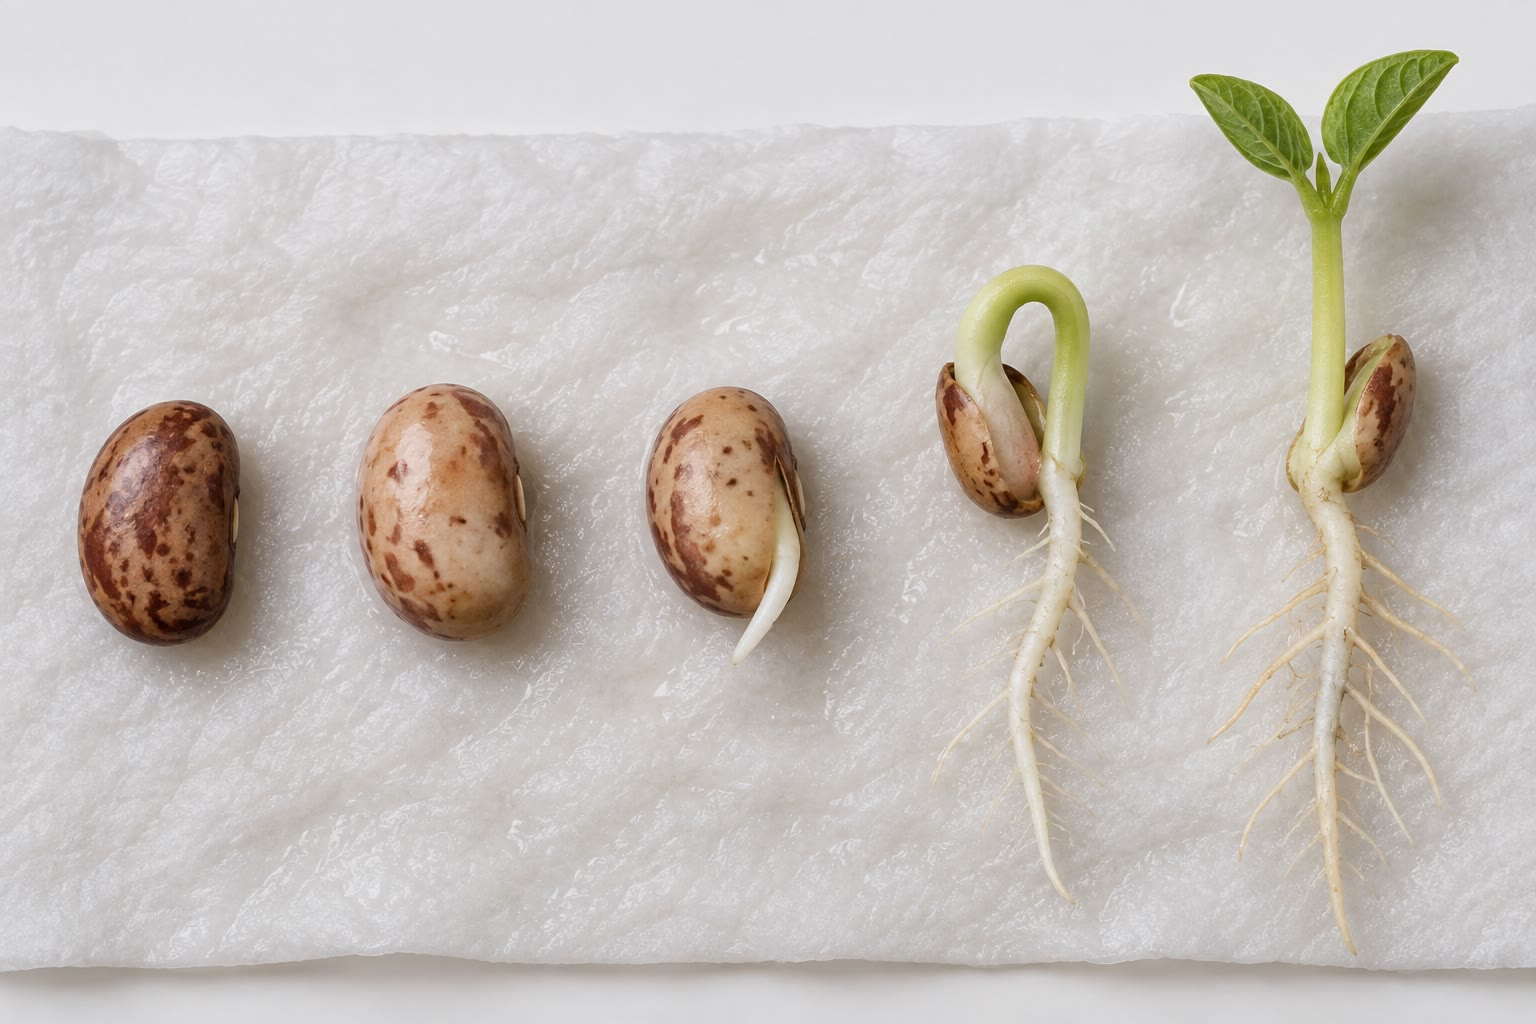
\includegraphics[width=0.66\linewidth]{images/book4/ai/b4-14-germinating-beans.jpg}

{\small 菜豆萌发：\omterm{def:b2:angiosperm-reproduction:seed}{种子}吸胀，胚根首先伸出，
下胚轴顶端的弯钩向上穿过土壤，
弯钩在光下伸直，第一片真叶展开。}
\end{omfigure}

\begin{theorem}[萌发作为一场赌博]\label{thm:b2:plant-flowering:bet}
\index{风险分散}
设每年萌发的\omterm{def:b2:angiosperm-reproduction:seed}{种子}占一批\omterm{def:b2:angiosperm-reproduction:seed}{种子}的比例为 $g$，
其余\omterm{def:b2:angiosperm-reproduction:seed}{种子}以概率 $s$ 在土壤中存活到下一年。在
良年中，一粒萌发的\omterm{def:b2:angiosperm-reproduction:seed}{种子}留下 $R_g$ 粒\omterm{def:b2:angiosperm-reproduction:seed}{种子}；在坏年中，
则不留下\omterm{def:b2:angiosperm-reproduction:seed}{种子}；每年为良年的概率为 $p$。一种策略
若一次性萌发全部\omterm{def:b2:angiosperm-reproduction:seed}{种子}（$g = 1$），则在多年的运行中，
其长期增长速率（取 $\ln$ 平均）为 $p\ln R_g + (1 - p)\ln 0 =
-\infty$：一个坏年便使其灭绝。当 $g < 1$ 时，策略
在良年中以因子 $gR_g + (1 - g)s$ 增长，在坏年中以
因子 $(1 - g)s > 0$ 增长，因此其长期速率，
\[
r = p\ln\bigl(gR_g + (1 - g)s\bigr) + (1 - p)\ln\bigl((1 - g)s\bigr),
\]
为有限值，且当 $p$ 不太接近 1 时，它在一个
中间的 $g$ 处取最大值。取 $R_g = 20$、$s = 0.8$、$p = 0.7$ 时，
最优值接近 $g = 0.7$：大部分萌发，留存一部分作为储备。
\omterm{def:b2:angiosperm-reproduction:seed}{休眠}并非萌发的失败，
而是演化形成的部分拒绝。
\end{theorem}
\begin{proof}
经过 $T$ 年后，种群大小为各年因子之积，
因此其增长速率即为各年因子对数的平均值
（几何平均速率），这正是选择在长期运行中最大化的量。
当 $g = 1$ 时，坏年因子为零，其对数为
$-\infty$。当 $g < 1$ 时两个因子均为正；对 $r$ 关于 $g$ 求导，
并令导数为零，即可得到最优解，
对所给数据，最优值位于 $g = 0.7$ 附近
（将 $r$ 在 $g = 0.4, 0.6, 0.8, 1$ 处取值，得 $1.28$、$1.42$、
$1.40$、$-\infty$）。
\end{proof}

\begin{omfigure}
\begin{tikzpicture}
\begin{axis}[
  width=0.7\linewidth, height=5.4cm,
  axis x line=bottom, axis y line=left,
  xmin=0, xmax=1, ymin=0, ymax=1.7,
  xlabel={每年萌发比例 $g$}, ylabel={长期增长速率 $r$},
  xlabel style={font=\small, at={(axis description cs:0.5,-0.13)}, anchor=north},
  ylabel style={font=\small},
  tick label style={font=\small}, xtick={0,0.2,0.4,0.6,0.8,1}, ytick={0,0.5,1,1.5},
  clip=false,
]
\addplot[very thick, omDef, domain=0.02:0.97, samples=100] {0.7*ln(20*x + 0.8*(1-x)) + 0.3*ln(0.8*(1-x))};
\draw[dashed, gray] (axis cs:0.7,0) -- (axis cs:0.7,1.43);
\node[font=\scriptsize, anchor=south] at (axis cs:0.7,1.45) {最优：\qty{30}{\%} 留在土壤中};
\node[font=\scriptsize, anchor=north west, align=left] at (axis cs:0.7,0.6) {$g \to 1$：一个坏年 \\使整批种子覆灭};
\end{axis}
\end{tikzpicture}

{\small \omterm{def:b2:angiosperm-reproduction:seed}{休眠}带来的\omterm{thm:b2:plant-flowering:bet}{风险分散}。十年中有七年为良年，
全部萌发的\omterm{def:b2:angiosperm-reproduction:seed}{种子}群体终将被一个坏年毁灭；
留存部分\omterm{def:b2:angiosperm-reproduction:seed}{种子}的群体，
长期增长最快。}
\end{omfigure}

\section{练习}

\begin{exercise}[$\star$]\label{exo:b2:plant-flowering:1}
区分营养\omterm{def:b2:plant-meristems:meristem}{分生组织}、\omterm{def:b2:plant-flowering:transition}{花序分生组织}和花\omterm{def:b2:plant-meristems:meristem}{分生组织}，
并说明其中哪些是有限生长的。
\end{exercise}

\begin{exercise}[$\star$]\label{exo:b2:plant-flowering:2}
给出\omterm{prop:b2:plant-flowering:photoperiod}{短日植物}、\omterm{prop:b2:plant-flowering:photoperiod}{长日植物}和日中性植物的定义，
各举一例，并说明\omterm{prop:b2:plant-flowering:photoperiod}{短日植物}实际测量的是什么。
\end{exercise}

\begin{exercise}[$\star$]\label{exo:b2:plant-flowering:3}
给出野生型及 ABC 模型三个单\omterm{def:b2:genome-diversification:mutation}{突变}体中各轮的
器官特征。
\end{exercise}

\begin{exercise}[$\star$]\label{exo:b2:plant-flowering:4}
列举四种打破\omterm{def:b2:angiosperm-reproduction:seed}{种子}\omterm{def:b2:angiosperm-reproduction:seed}{休眠}的信号，并对每一种说明它所反映的季节
或地点。
\end{exercise}

\begin{exercise}[$\star\star$]\label{exo:b2:plant-flowering:5}
某\omterm{prop:b2:plant-flowering:photoperiod}{短日植物}的临界夜长为 \qty{10}{h}。判断它
在以下条件下是否开花：\qty{16}{h} 光照/\qty{8}{h} 黑暗；\qty{12}{h}/\qty{12}{h}；
\qty{12}{h} 光照、\qty{6}{h} 黑暗，再加一分钟光照、\qty{6}{h} 黑暗；
\qty{8}{h} 光照、\qty{4}{h} 黑暗，再 \qty{4}{h} 光照、\qty{8}{h} 黑暗。
\end{exercise}

\begin{exercise}[$\star\star$]\label{exo:b2:plant-flowering:6}
将已诱导的\omterm{prop:b2:plant-flowering:photoperiod}{短日植物}的一片叶嫁接到
长日条件下生长的\omterm{prop:b2:plant-flowering:photoperiod}{长日植物}上，该\omterm{prop:b2:plant-flowering:photoperiod}{长日植物}开花。这说明开花素
有何性质？若嫁接所用的叶
已被诱导，但叶柄处的韧皮部被切断，
结果又如何？
\end{exercise}

\begin{exercise}[$\star\star$]\label{exo:b2:plant-flowering:7}
寒冷使阻遏物以每天 $\alpha = 0.05$ 的速率失活，
而开花需要 $f < 0.15$。需要多少个寒冷日？某个
冬季有三段寒冷期，分别为 15、12 和 20 天，中间
隔以回暖：该植物是否经历了春化？若 $\alpha$ 为 $0.02$，结果又如何？
\end{exercise}

\begin{exercise}[$\star\star$]\label{exo:b2:plant-flowering:8}
从染色质的角度解释，经春化的植物为何在
其\omterm{def:b2:angiosperm-reproduction:seed}{种子}中丢失“记忆”，以及这为何有用。
\end{exercise}

\begin{exercise}[$\star\star$]\label{exo:b2:plant-flowering:9}
在黑暗中依次给莴苣\omterm{def:b2:angiosperm-reproduction:seed}{种子}照射以下光照序列：R；R 后接 FR；
R、FR、R；R、FR、R、FR。预测每种情况下\omterm{def:b2:angiosperm-reproduction:seed}{种子}是否萌发，并
用两种形式的\omterm{prop:b2:plant-flowering:photoperiod}{光敏色素}加以解释。
\end{exercise}

\begin{exercise}[$\star\star\star$]\label{exo:b2:plant-flowering:10}
在风险分摊模型中，取 $R_g = 20$，$s = 0.8$，计算
$g = 0.4$、$0.6$、$0.8$ 和 $1$ 时的长期增长速率，
当 $p = 0.7$ 时，再计算 $p = 0.95$ 时的结果。最优值如何移动，
这对沙漠与草地各预测什么？
\end{exercise}

\begin{exercise}[$\star\star\star$]\label{exo:b2:plant-flowering:11}
预测以下情形产生的花：在四轮中都表达 B 类基因；
在四轮中都表达 C 类基因；由双\omterm{def:b2:genome-diversification:mutation}{突变}体
缺失 A 和 B 产生。随后解释缺失 C 的花为何
仍会继续形成若干轮结构。
\end{exercise}

\begin{exercise}[$\star\star\star$]\label{exo:b2:plant-flowering:12}
“植物通过整合自己无法控制的信号
来决定开花。”讨论本章的三种整合：日长、
寒冷，以及\omterm{def:b2:angiosperm-reproduction:seed}{种子}库中的年份，并说明整合
机制使植物免受哪些风险，这是简单阈值
所不能防范的。
\end{exercise}

\section{问题：种植者的日历}

\begin{problem}[{周末问题——菊花种植者用灯光安排开花，小麦育种者统计寒冷，
花店的重瓣花得到解释，一批种子的休眠被建模，
最终落在触发作物开花的夜长、
小麦所需的寒冷日数，以及
最佳萌发比例上}]
\label{pb:b2:plant-flowering:1}
菊花为\omterm{prop:b2:plant-flowering:photoperiod}{短日植物}，其临界夜长为
\qty{9.5}{h}；诱导需要连续 \num{12} 个诱导性
夜晚，诱导后 \num{8} 周开花。十一月
温室在 17:00 至 07:30 处于黑暗中。冬小麦
每个寒冷日 $\alpha = 0.06$，当 $f < 0.10$ 时开花。\omterm{def:b2:angiosperm-reproduction:seed}{种子}
批次：$R_g = 15$，$s = 0.7$，丰年出现的概率为 $p$。

\medskip
\noindent\textbf{第一部分——温室。}
\begin{enumerate}
  \item 六月自然夜长为 \qty{8}{h}，作物
        能否开花？种植者若要在八月出售花卉，须怎样做？
  \item 种植者用黑布将作物从
        每晚 19:00 罩到 07:00。植物所感受的夜长为多少？
        若要使作物在
        8 月 15 日开花，遮盖应从何时开始？
  \item 十一月自然夜长为 \qty{14}{h}，种植者希望
        将开花\emph{推迟}到圣诞节。请设计一套光照方案，
        并解释为何短暂的闪光即已足够。
  \item 闪光在 21:00 而非
        00:00 给出，诱导并未被阻止。请结合
        临界夜长加以解释。
  \item 十二个夜晚中有一晚未盖黑布。请预测，
        并说明苍耳本会如何表现。
  \item 闪光以绿光给出时失效，以红光给出时
        有效；红光后接远红光则失效。请加以解释。
  \item 将已诱导植物的一片单叶嫁接到
        处于长日条件下的植物上。请预测结果，并说明它能证明什么。
\end{enumerate}

\medskip
\noindent\textbf{第二部分——小麦。}
\begin{enumerate}[resume]
  \item 小麦需要多少个寒冷日？
  \item 十月播种，十一月获得 10 个寒冷日，
        十二月气温温和，一月获得 25 个，二月获得 12 个。
        它在何时完成春化？
  \item 三月播种，获得 6 个寒冷日。它当年
        夏天会开花吗？这对农业生产有何影响？
  \item 某\omterm{def:b2:genome-diversification:mutation}{突变}体缺失阻遏物。请预测其表现，并说明
        育种者为何将这类小麦称为“春小麦”。
  \item 请解释寒冷的“记忆”为何能经受春季\omterm{def:b2:plant-meristems:meristem}{分生组织}的
        分裂而保留，却无法经受形成下一代的
        \omterm{def:b2:meiosis-heredity:meiosis}{减数分裂}。
  \item 为何寒冷必须在\omterm{def:b2:plant-meristems:meristem}{分生组织}中计数，
        而不像日长那样在叶中计数？
\end{enumerate}

\medskip
\noindent\textbf{第三部分——花艺师。}
\begin{enumerate}[resume]
  \item 重瓣玫瑰的\omterm{def:b2:angiosperm-reproduction:flower}{雄蕊}位置长有花瓣，花心
        处还多出几片花瓣。哪一类基因功能缺失？
        写出轮式公式。
  \item 此类玫瑰作为\omterm{def:b2:plant-life-cycles:heterospory}{花粉}亲本不育，
        但有时仍能结实。请用 ABC 模型解释这两个事实。
  \item 一株金鱼草的\omterm{def:b2:angiosperm-reproduction:flower}{雄蕊}代替了花瓣，\omterm{def:b2:angiosperm-reproduction:flower}{心皮}
        代替了萼片。哪一类基因功能缺失？
  \item 预测一株在第 1 轮中也表达 C 类基因、
        其余各轮正常的植物的花。
  \item 为何相同的\omterm{def:b2:genome-diversification:mutation}{突变}会在玫瑰、金鱼草
        和\emph{Arabidopsis}中产生相同的转变，
        这些植物相隔约一亿年？
  \item 在野生型花的第 2 轮中，A 与 B 均有活性。
        若只有 B 在该处有活性，预测该处的器官。
\end{enumerate}

\medskip
\noindent\textbf{第四部分——\omterm{def:b2:angiosperm-reproduction:seed}{种子}批次。}
\begin{enumerate}[resume]
  \item 计算长期增长速率 $r$，取 $g = 0.5$、$0.7$
        与 $0.9$，且 $p = 0.8$。
  \item 三者中哪一个最好？$g = 1$ 时会发生什么？
  \item 对 $p = 0.5$（沙漠）重新计算。现在哪一个 $g$ 最好？
  \item 种植者在好年景将整批\omterm{def:b2:angiosperm-reproduction:seed}{种子}播于同一块田中，
        每粒\omterm{def:b2:angiosperm-reproduction:seed}{种子}收获 $R_g$。解释其策略为何不同于植物，
        以及他要如何做才能保住该品种，
        使其度过坏年景。
  \item 这些\omterm{def:b2:angiosperm-reproduction:seed}{种子}萌发需要光照。解释这一特性对一粒小\omterm{def:b2:angiosperm-reproduction:seed}{种子}的
        适应意义，并预测翻耕
        对\omterm{def:b2:angiosperm-reproduction:seed}{种子}库有何影响。
  \item 给出结论：临界夜长与覆盖时间表、
        小麦的寒冷需求量，以及最好的 $g$ 值
        （分别对应 $p = 0.8$ 与 $p = 0.5$）。
\end{enumerate}
\end{problem}
